\documentclass[a4paper]{article}

\usepackage[utf8]{inputenc}
\usepackage[T1]{fontenc}
\usepackage[french]{babel}
\usepackage{fullpage}
\usepackage{hyperref}
\usepackage{amsmath}
\usepackage{amssymb}
\usepackage{upgreek}
\usepackage{color}
\usepackage[]{algorithm2e}
\usepackage{stmaryrd}
\usepackage{graphicx}
\usepackage{float}
\usepackage{multirow}
\usepackage{subfig}
\usepackage[table]{xcolor}
\title{
    Assignment 3 : Multi-Armed Bandits\\
    \small INFO-F-409 - Learning Dynamics
}
\author{Florentin \bsc{Hennecker} (ULB 000382078)}
\date{}


\begin{document}
\maketitle

\section{N-Armed Bandit}
\subsection{Exercise 1}

Let us compare the performance of several algorithms trying to maximise the
reward they receive from an N-armed bandit which has 4 arms, each of which 
producing a reward sampled from a normal distribution of which the parameters
are shown in table \ref{banditparams}.

\begin{table}[H]
\centering
\begin{tabular}{c|c|c}
	\textbf{Arm} & $\mu$ & $\sigma$ \\
	\hline
	1 & 2.3 & 0.9\\
	2 & 2.1 & 0.6\\
	3 & 1.5 & 0.4\\
	4 & 1.3 & 2\\
\end{tabular}
\caption{Parameters of the 4-armed bandit}
\label{banditparams}
\end{table}

The algorithms to compare are $\epsilon$-greedy with parameters 0, 0.1 and 0.2,
Softmax with temperatures 1 and 0.1, and the random action selection policy.
Figure \ref{ex11perf} shows how each of these algorithms manage to maximise
their reward after playing for many iterations. 
\begin{figure}[H]
	\centering
	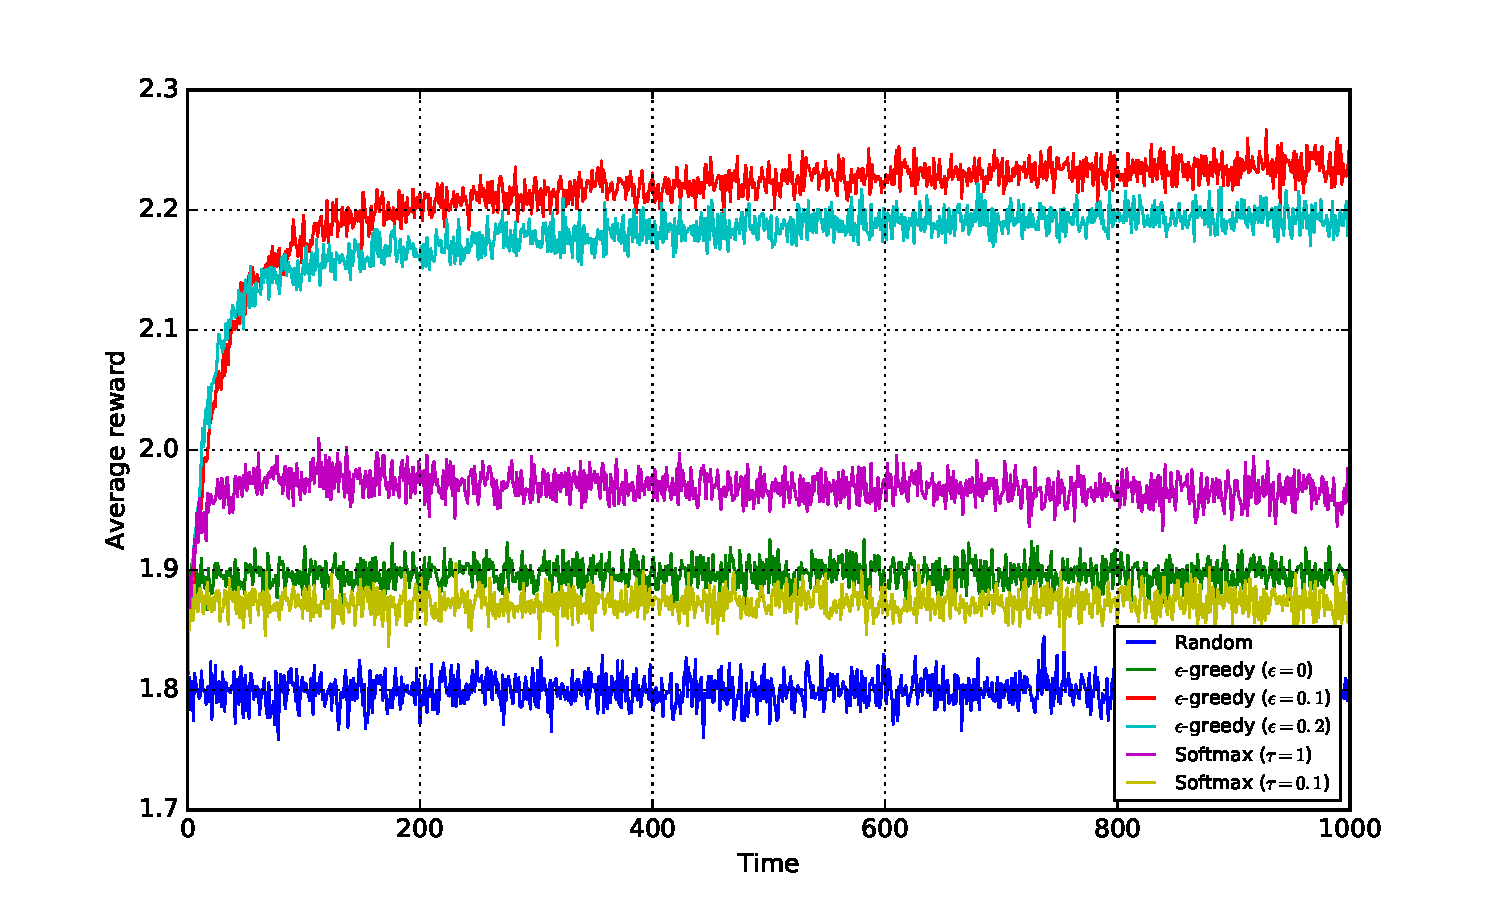
\includegraphics[width=0.7\textwidth]{./fig/ex1-1.pdf}
	\caption{Evolution of the average reward over 3000 runs during training}
	\label{ex11perf}
\end{figure}
As we can see, only two algorithms managed to converge to the best arm : 
$\epsilon$-greedy 0.1 and 0.2. Let us first explain the behaviour of 
$\epsilon$-greedy 0. It selects its first action at random, but for all the
following iterations, it will choose it again as its Q-value will be non-zero
and there is no room to explore. If all the arms had negative $Q*_{ai}$, 
$\epsilon$-greedy would however pick the less negative one after it has explored
all of the actions.\\

Softmax outperforms the random selection policy but does not do very well. 
This is likely caused by the fact that there is a lot of noise in the rewards
and that the discrete distribution regulating the choice of action is fairly
homogeneous. 

\begin{figure}[H]
	\centering
	\subfloat[][Arm 1]{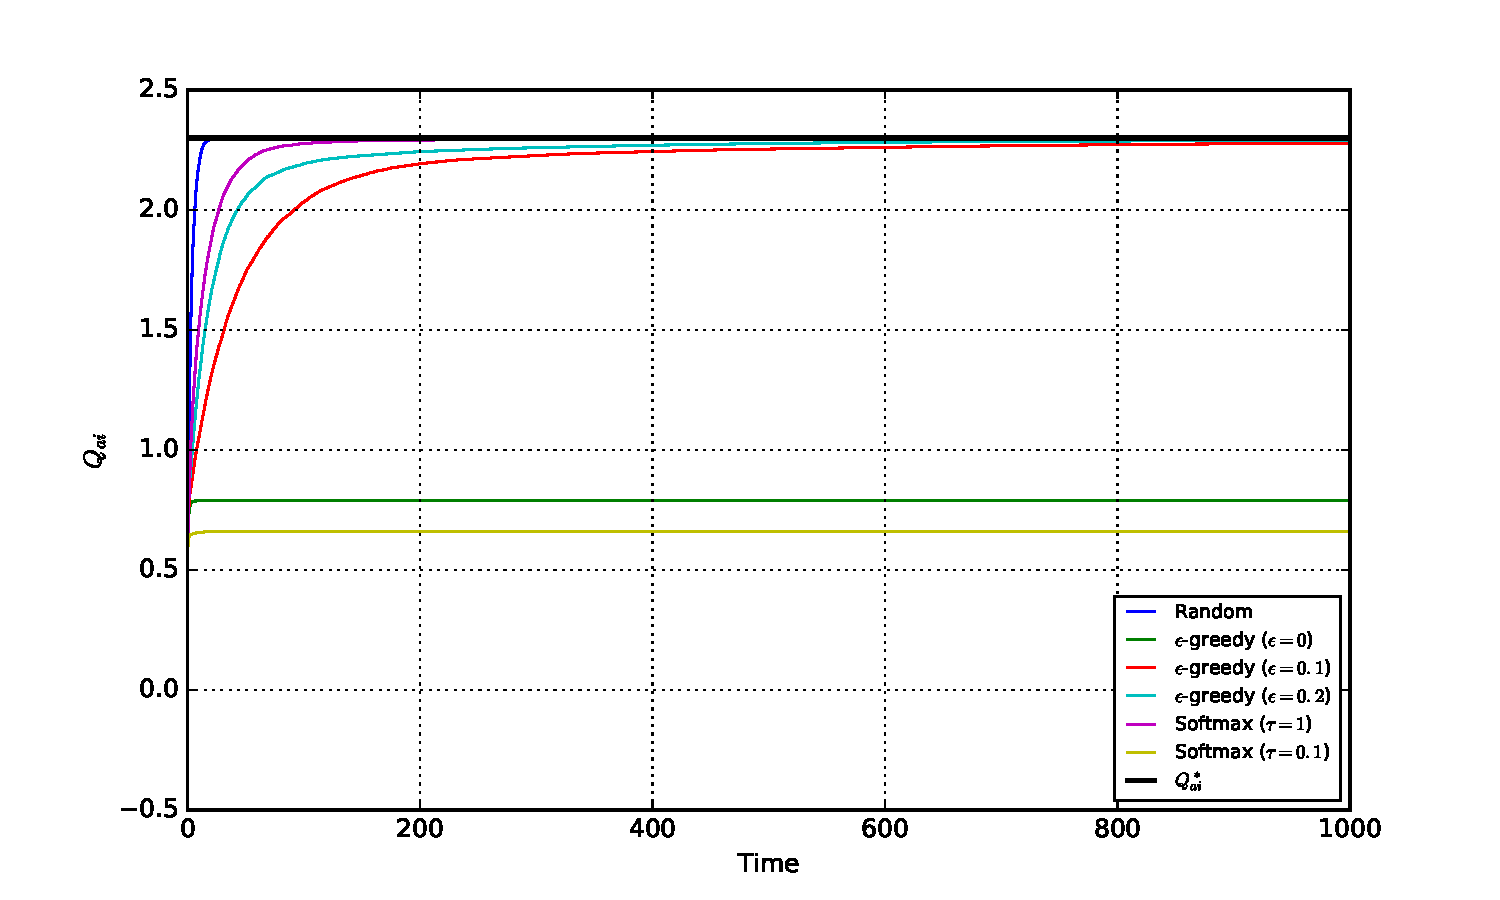
\includegraphics[width=.49\textwidth]{./fig/ex1-1-q0.pdf}}
	\subfloat[][Arm 2]{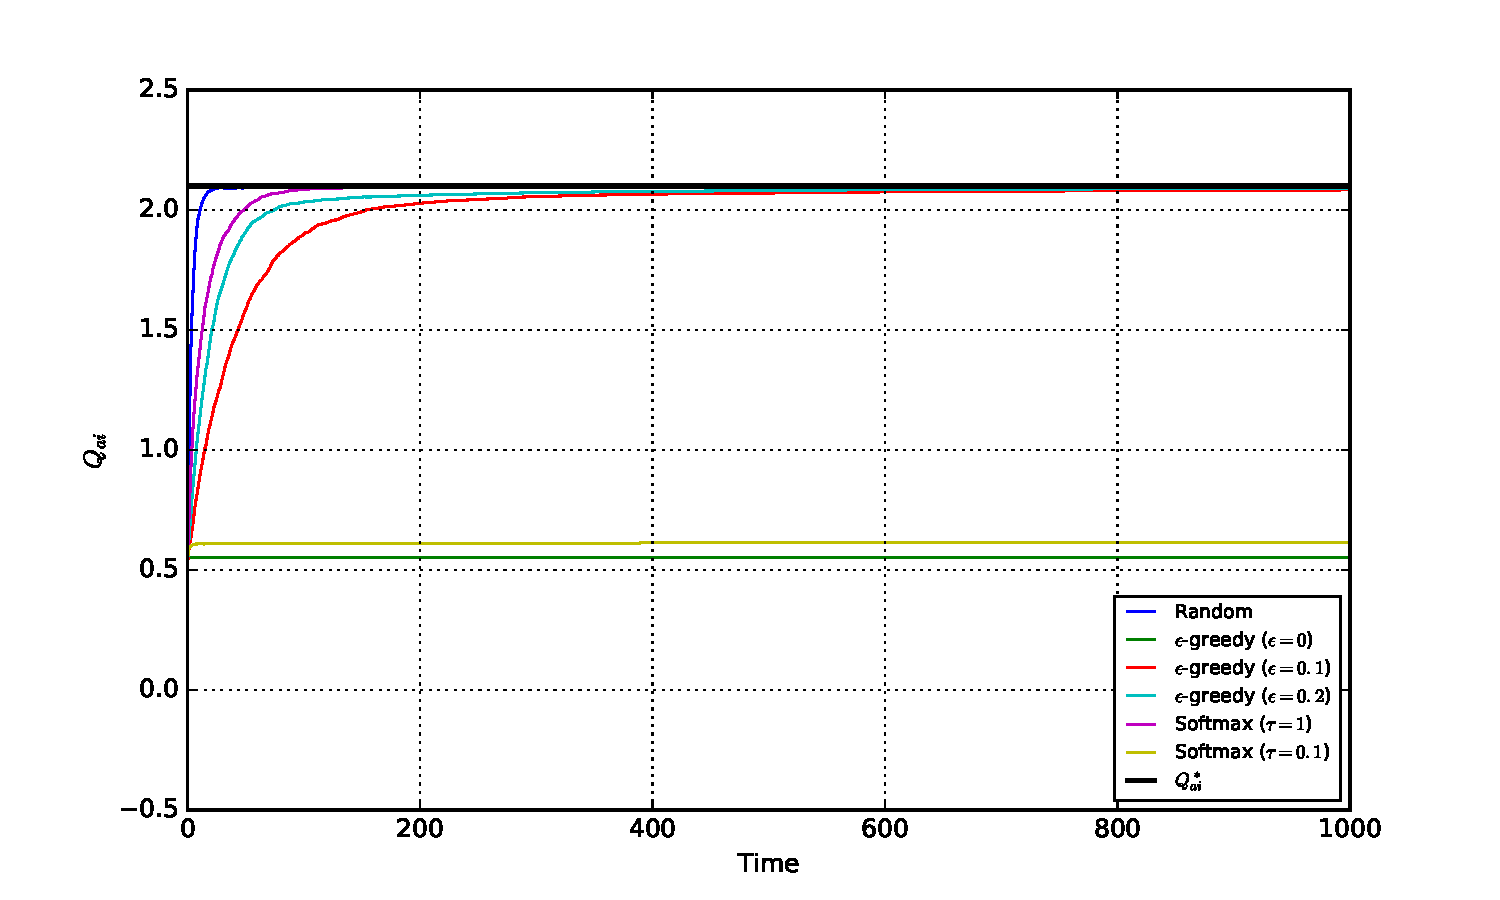
\includegraphics[width=.49\textwidth]{./fig/ex1-1-q1.pdf}}
	\\
	\subfloat[][Arm 3]{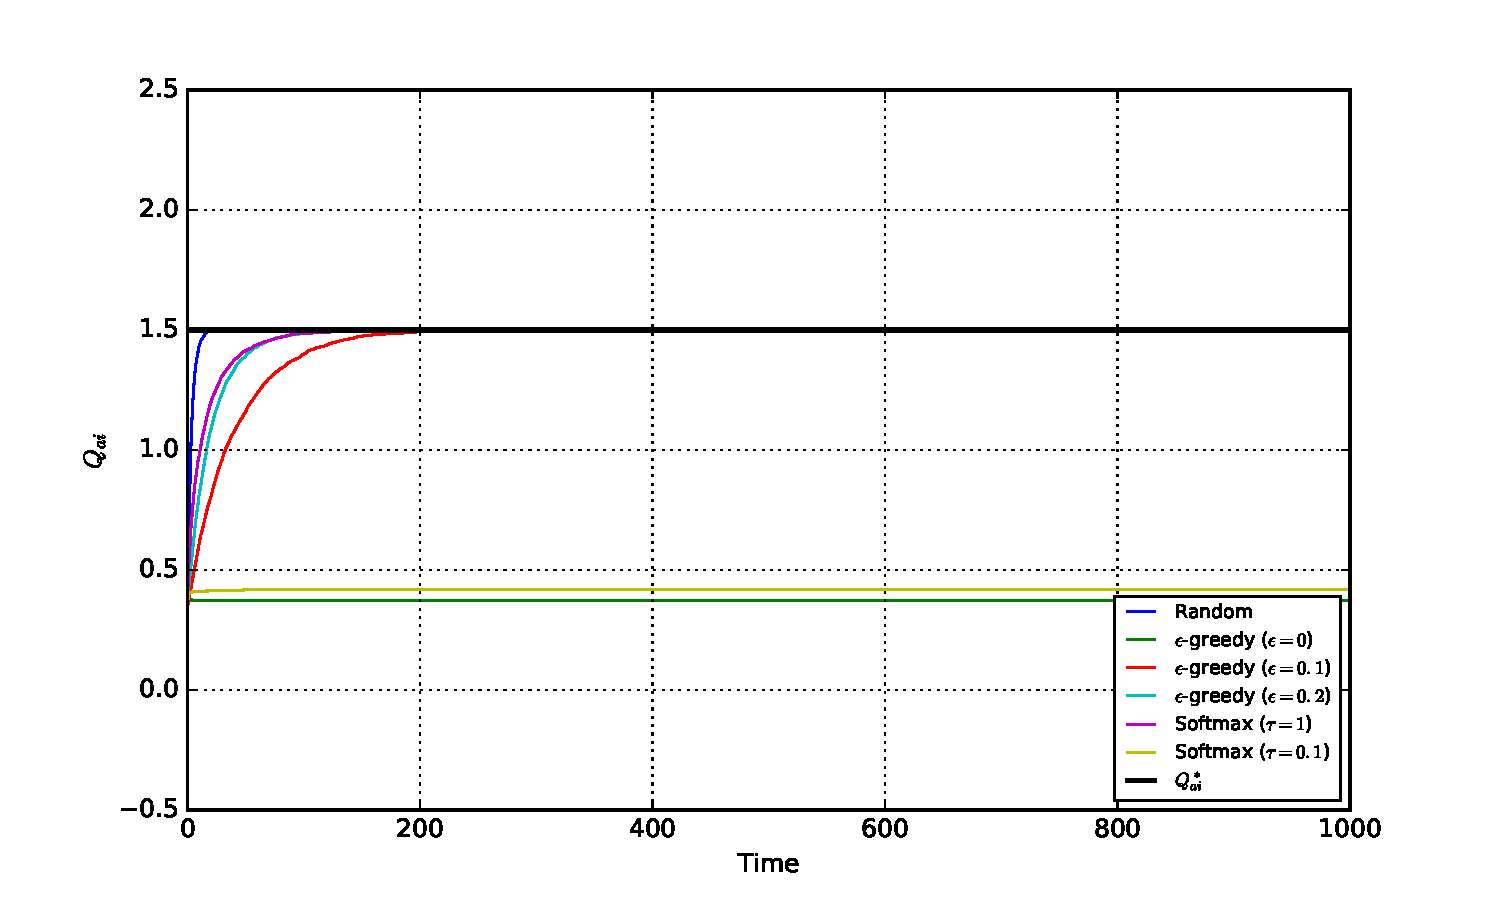
\includegraphics[width=.49\textwidth]{./fig/ex1-1-q2.pdf}}
	\subfloat[][Arm 4]{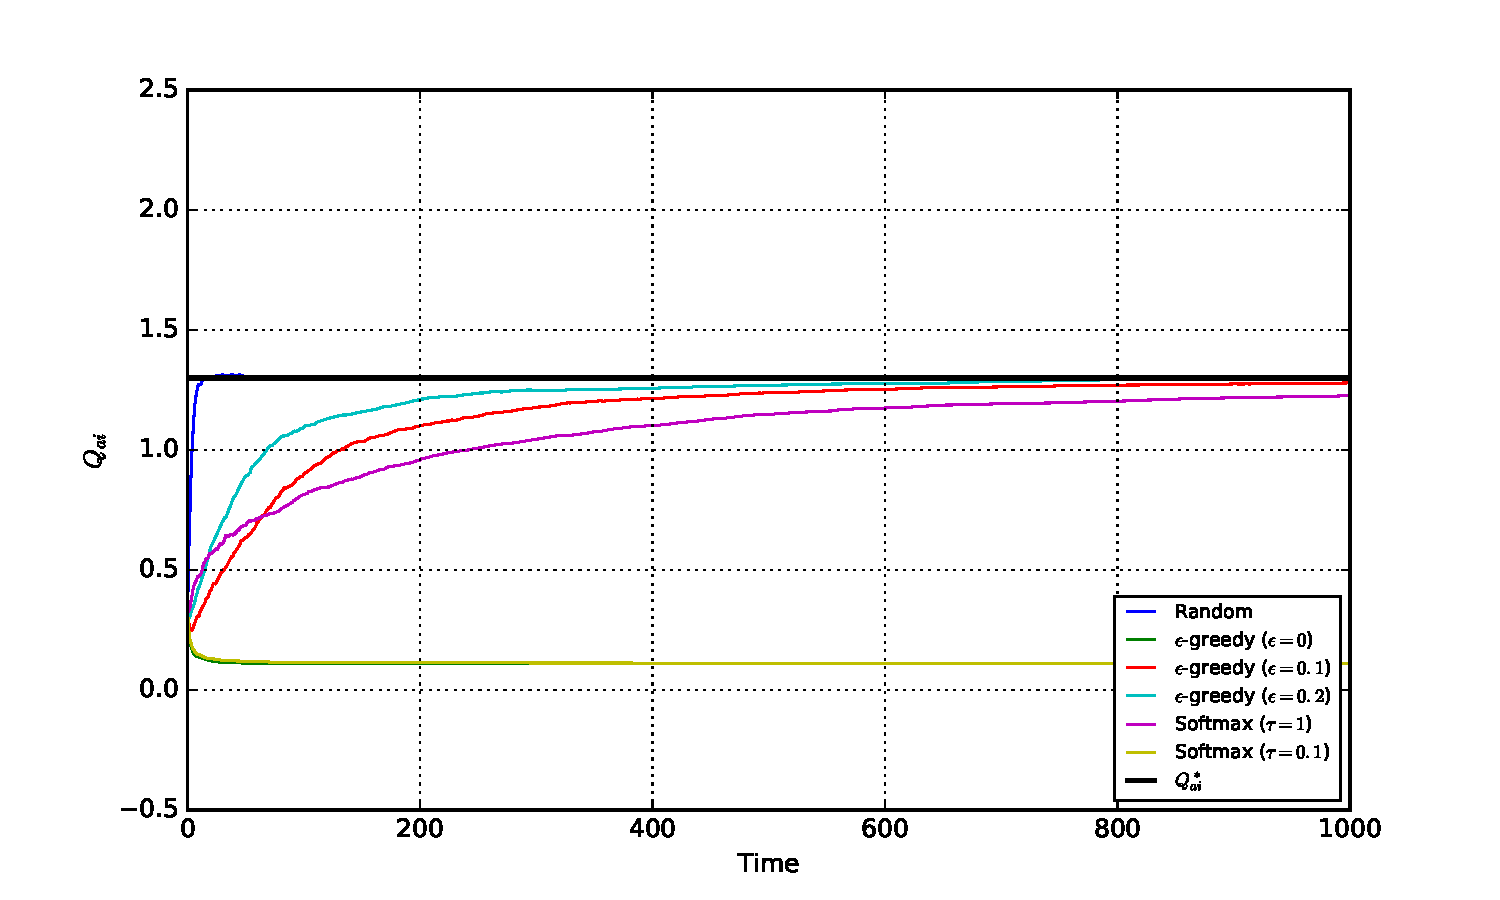
\includegraphics[width=.49\textwidth]{./fig/ex1-1-q3.pdf}}
	\caption{Evolution of $Q_{ai}$ for each arm}
	\label{ex11q}
\end{figure}

\begin{figure}[H]
	\centering
	\subfloat[][Random]{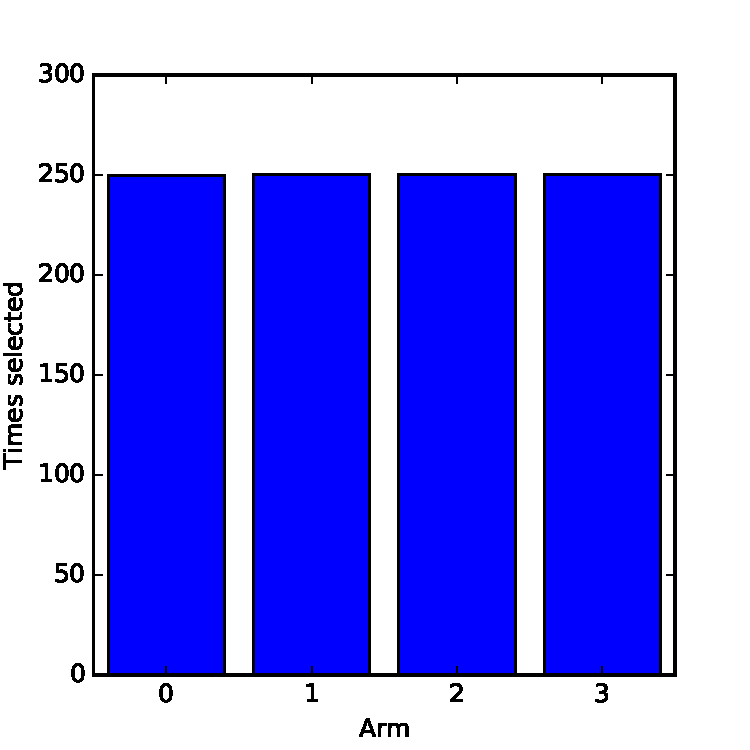
\includegraphics[width=.16\textwidth]{./fig/ex1-1-a0.pdf}}
	\subfloat[][$\epsilon$-greedy 0]{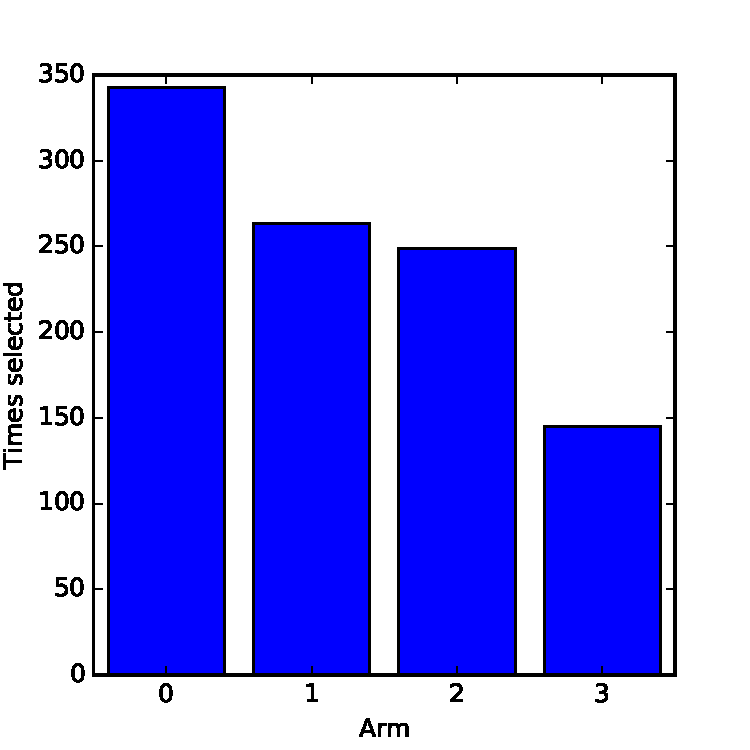
\includegraphics[width=.16\textwidth]{./fig/ex1-1-a1.pdf}}
	\subfloat[][$\epsilon$-greedy 0.1]{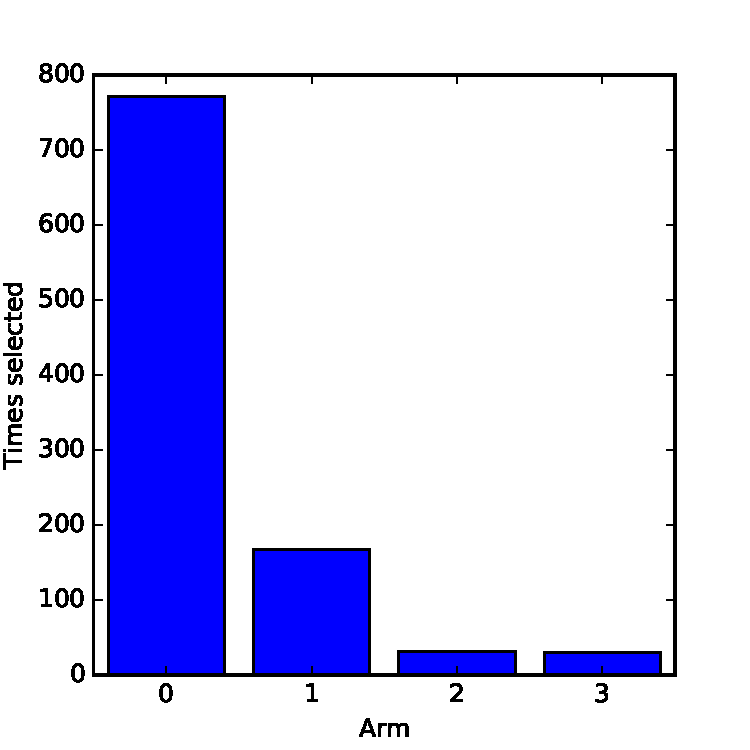
\includegraphics[width=.16\textwidth]{./fig/ex1-1-a2.pdf}}
	\subfloat[][$\epsilon$-greedy 0.2]{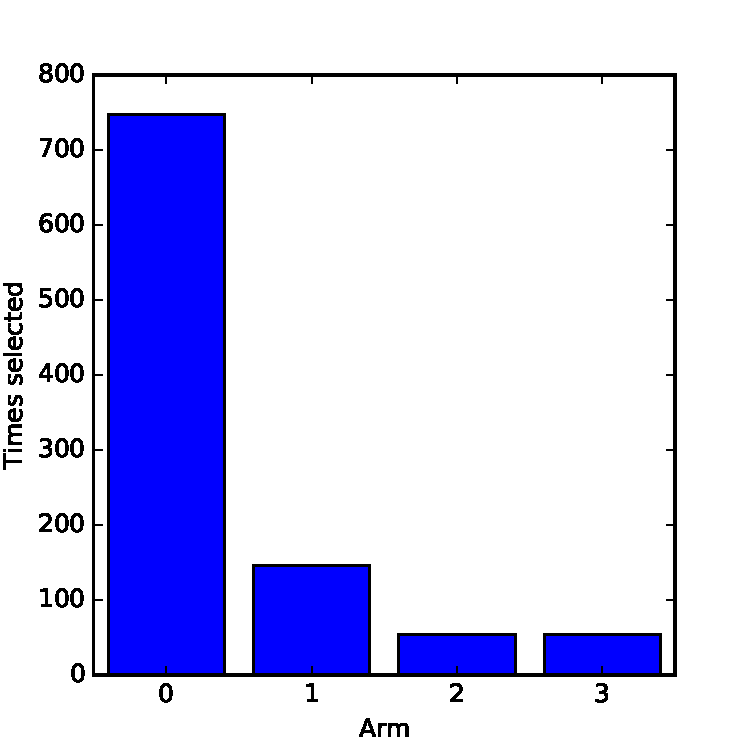
\includegraphics[width=.16\textwidth]{./fig/ex1-1-a3.pdf}}
	\subfloat[][Softmax 1]{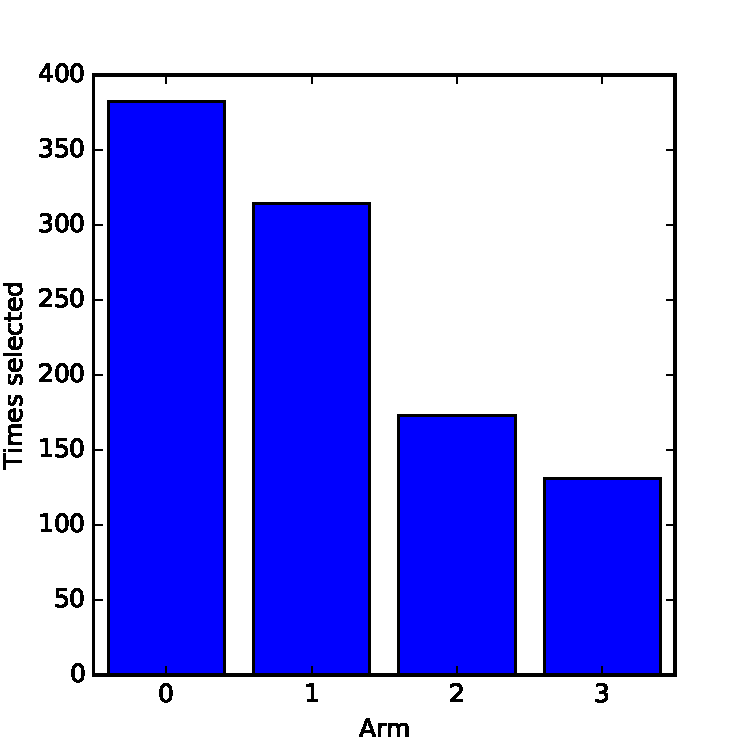
\includegraphics[width=.16\textwidth]{./fig/ex1-1-a4.pdf}}
	\subfloat[][Softmax 0.1]{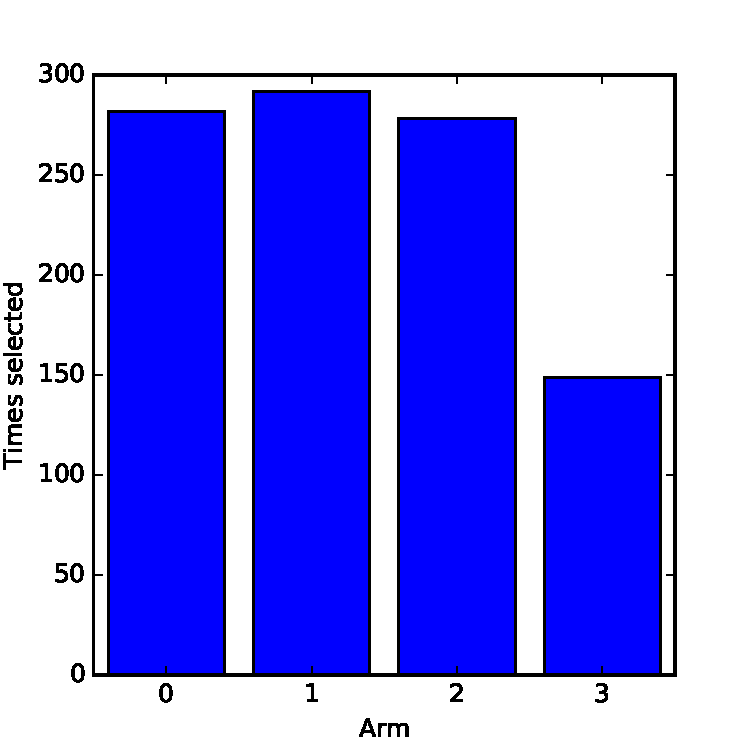
\includegraphics[width=.16\textwidth]{./fig/ex1-1-a5.pdf}}
	\caption{Actions taken by each algorithm}
	\label{ex11a}
\end{figure}

\begin{figure}[H]
	\centering
	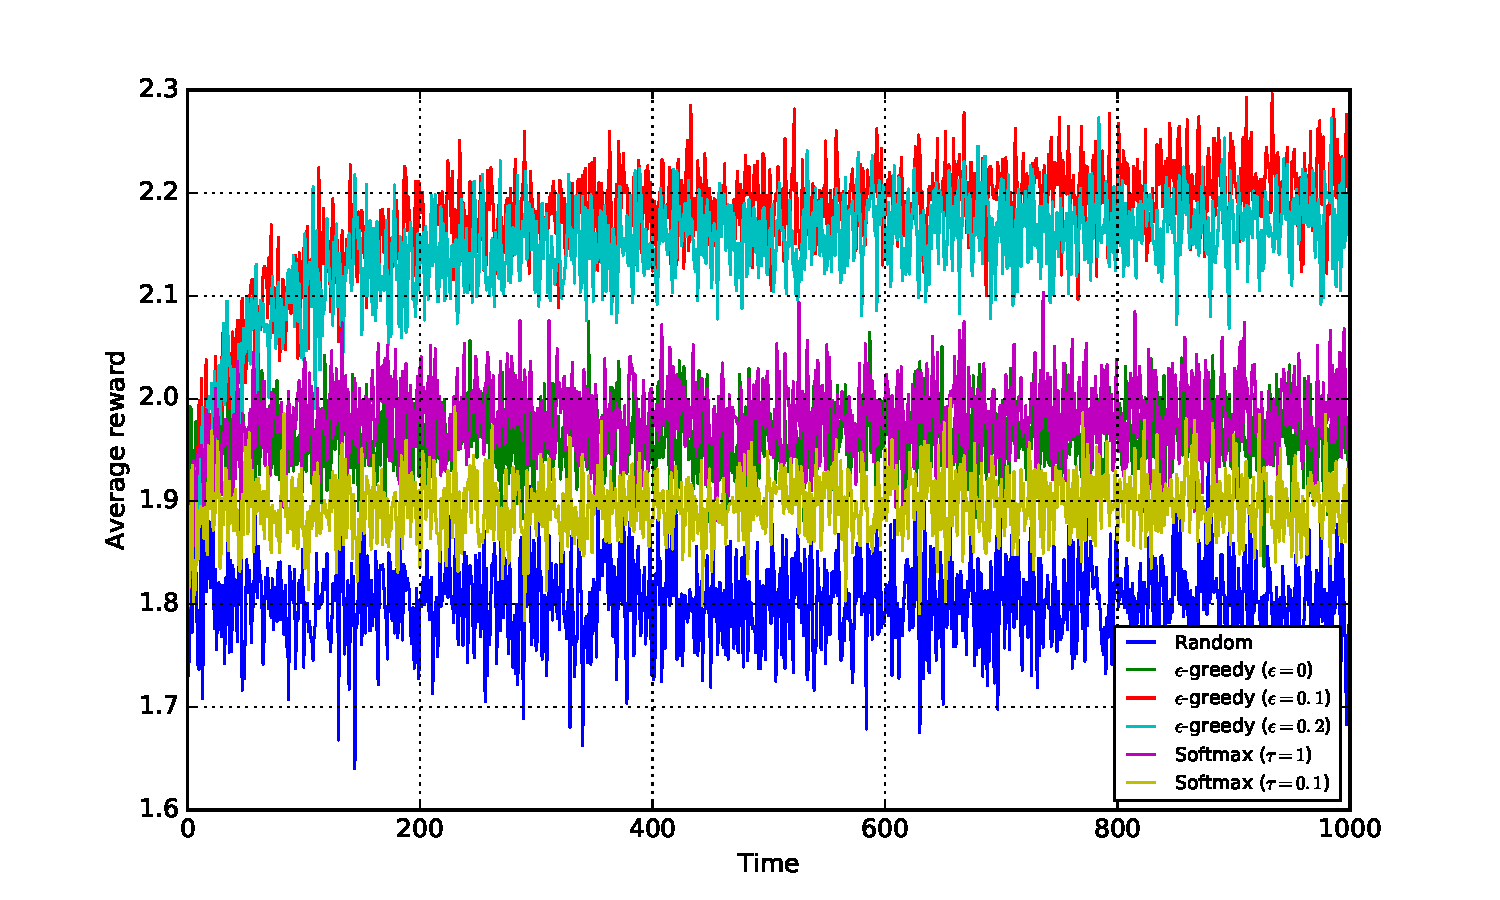
\includegraphics[width=0.7\textwidth]{./fig/ex1-2.pdf}
	\caption{Evolution of the average reward over 3000 runs during training}
	\label{ex12perf}
\end{figure}
\begin{figure}[H]
	\centering
	\subfloat[][Arm 1]{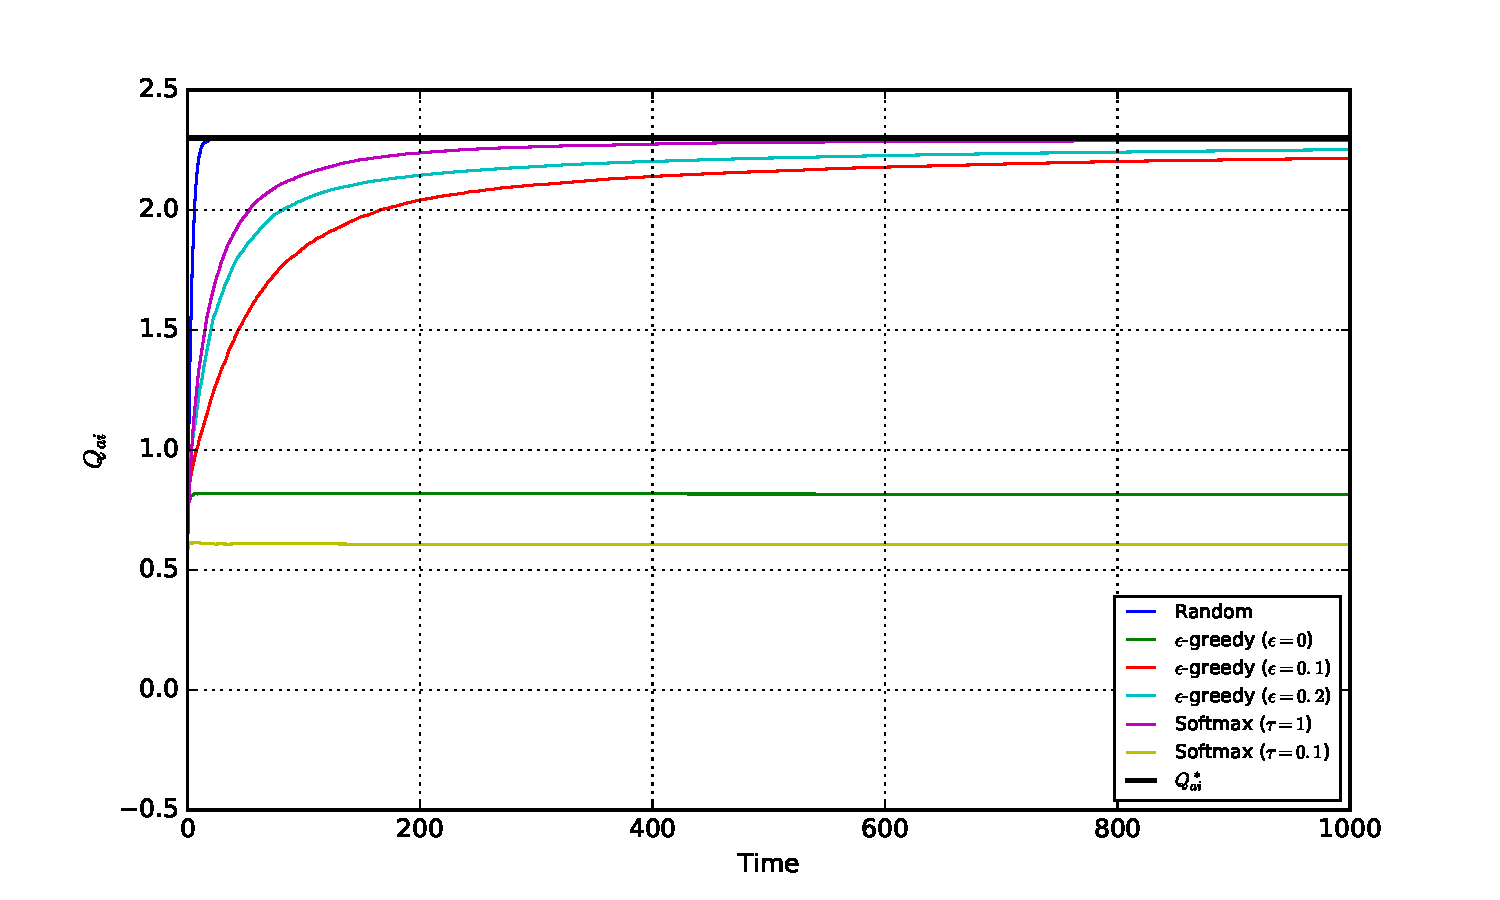
\includegraphics[width=.49\textwidth]{./fig/ex1-2-q0.pdf}}
	\subfloat[][Arm 2]{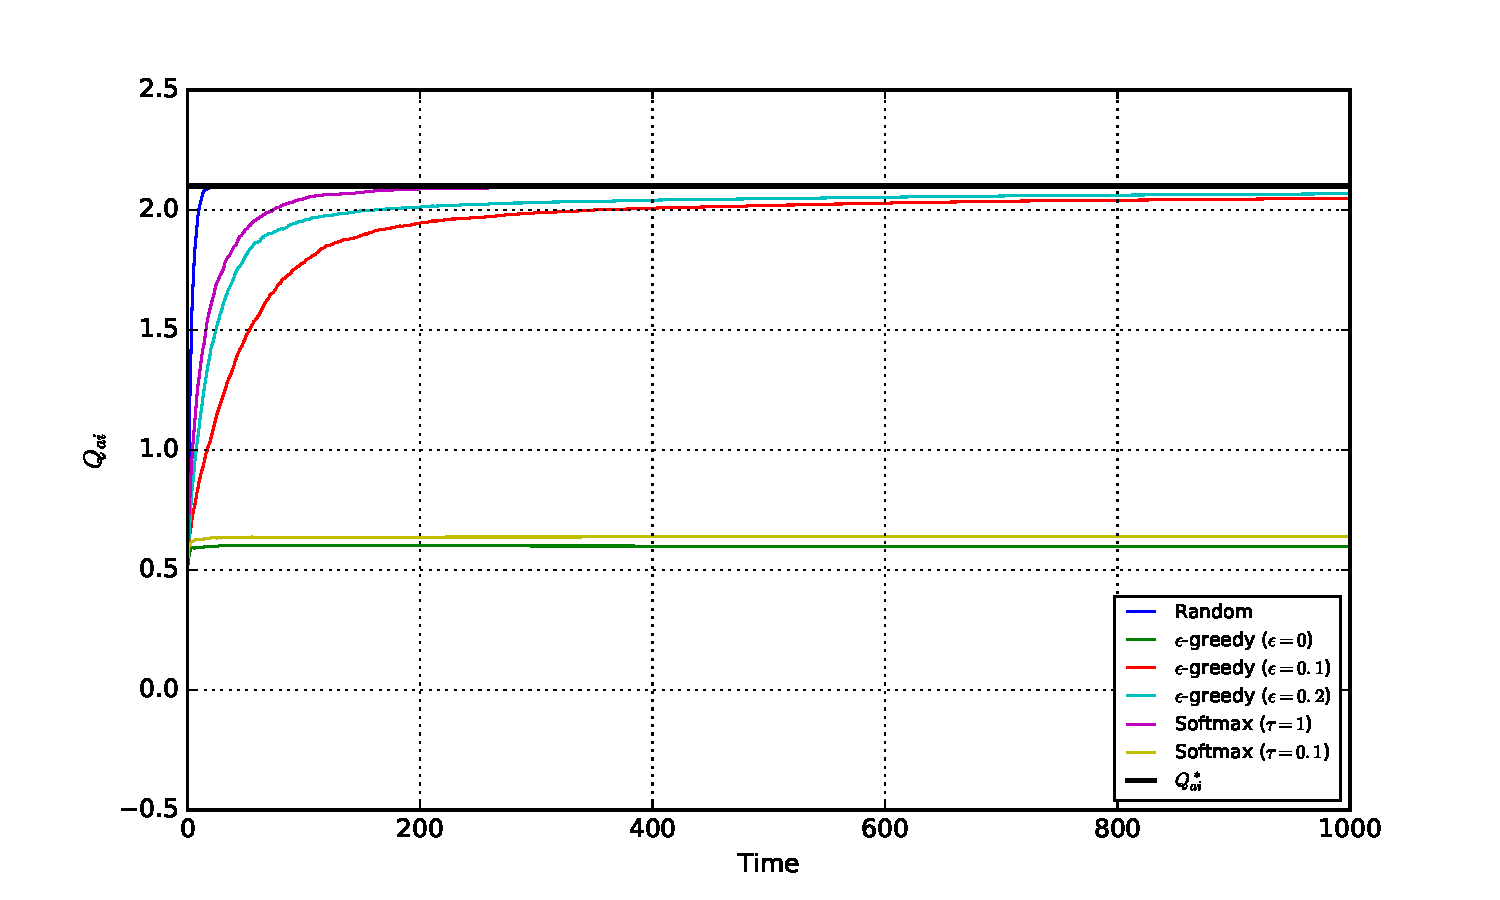
\includegraphics[width=.49\textwidth]{./fig/ex1-2-q1.pdf}}
	\\
	\subfloat[][Arm 3]{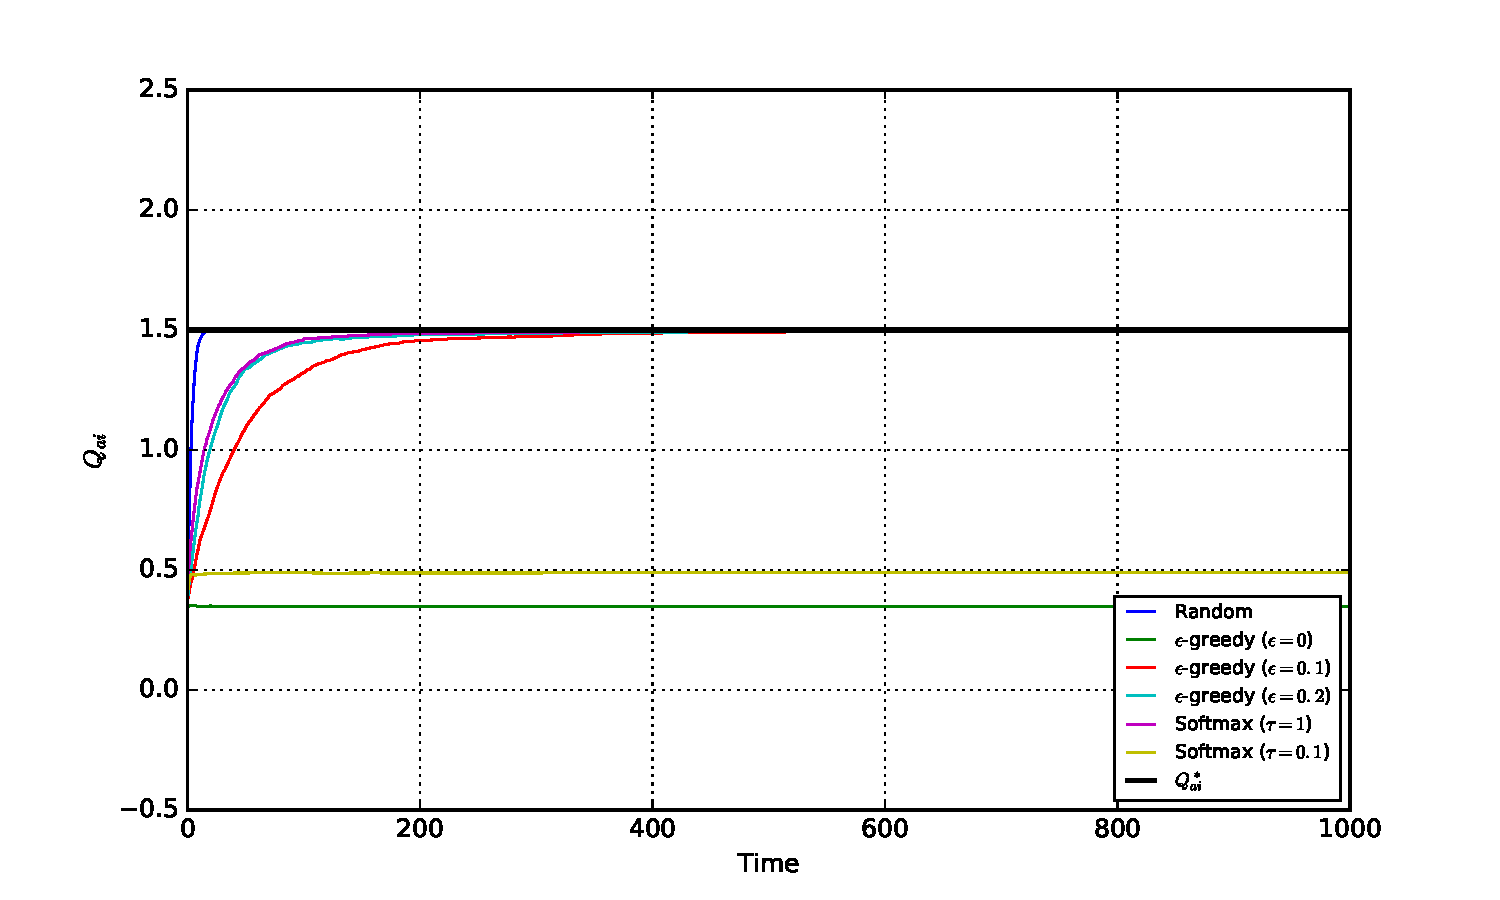
\includegraphics[width=.49\textwidth]{./fig/ex1-2-q2.pdf}}
	\subfloat[][Arm 4]{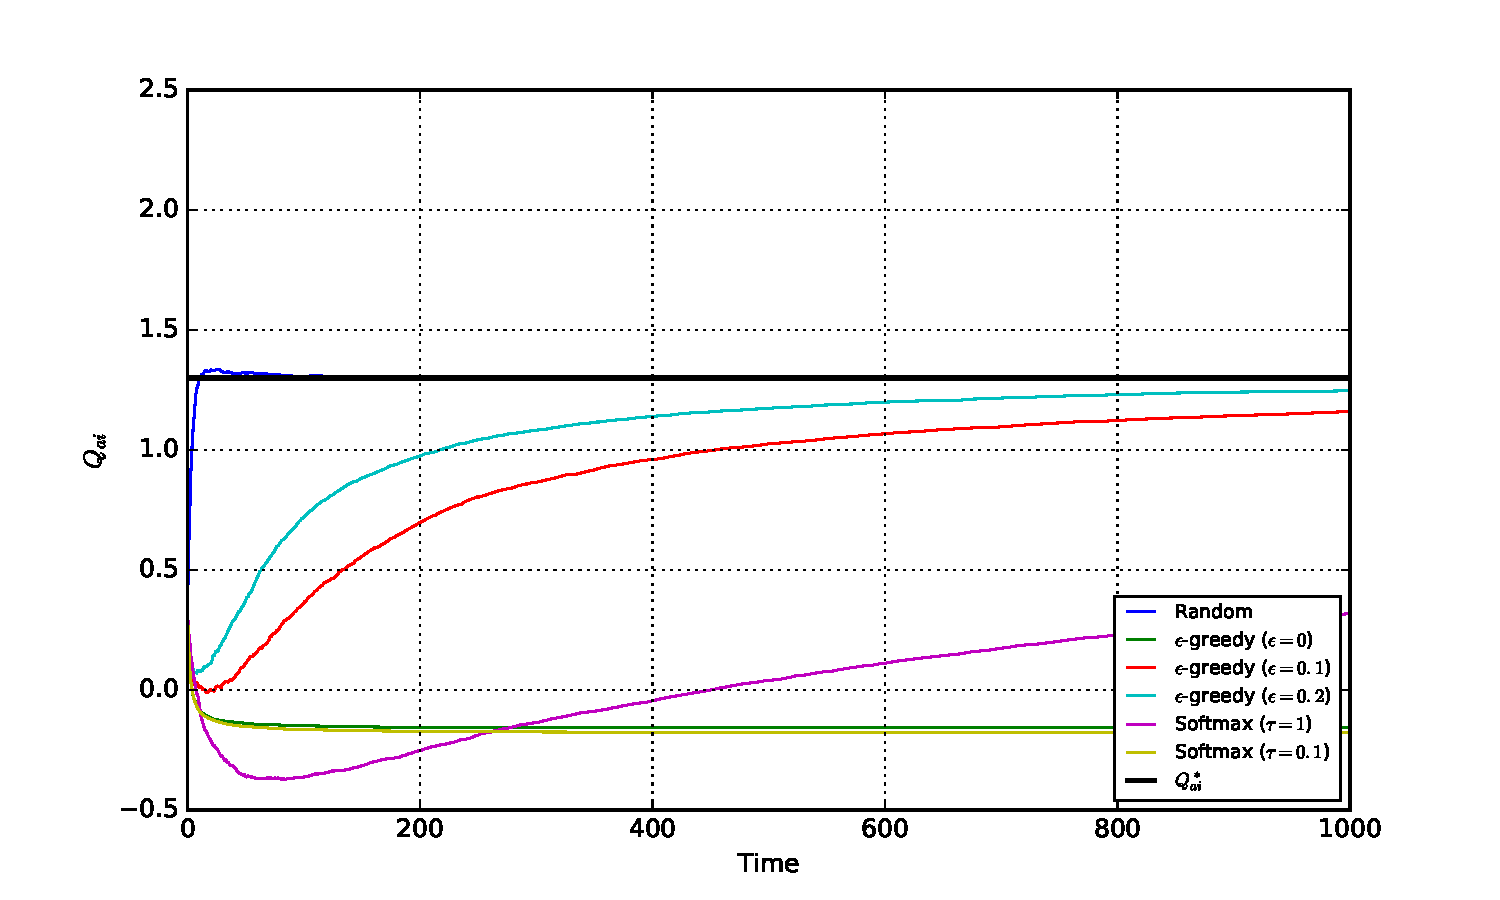
\includegraphics[width=.49\textwidth]{./fig/ex1-2-q3.pdf}}
	\caption{Evolution of $Q_{ai}$ for each arm}
	\label{ex12q}
\end{figure}
\begin{figure}[H]
	\centering
	\subfloat[][Random]{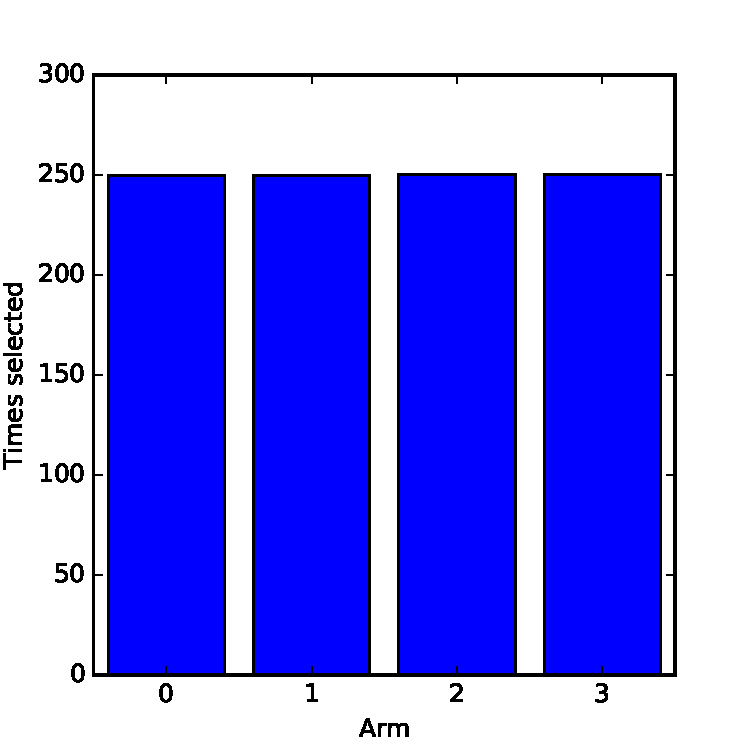
\includegraphics[width=.16\textwidth]{./fig/ex1-2-a0.pdf}}
	\subfloat[][$\epsilon$-greedy 0]{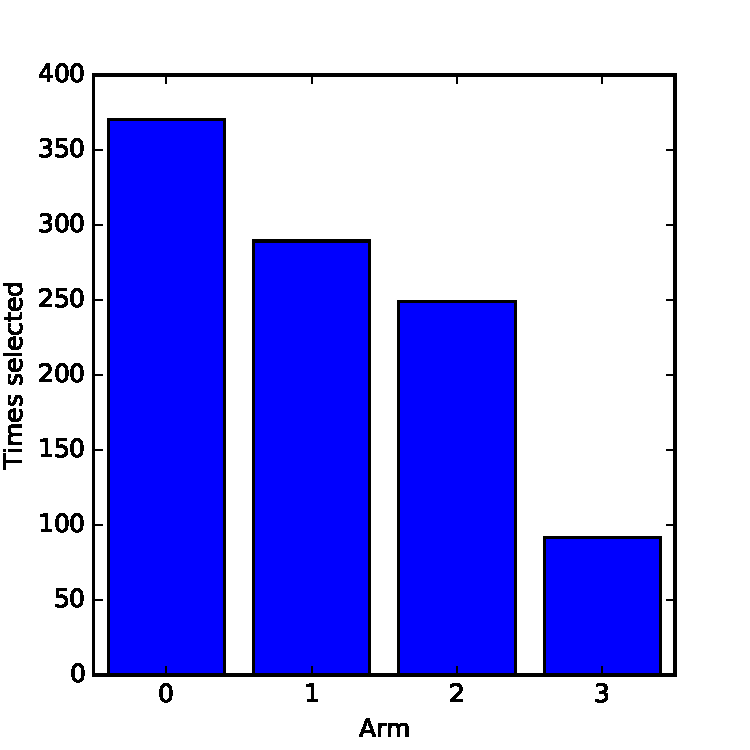
\includegraphics[width=.16\textwidth]{./fig/ex1-2-a1.pdf}}
	\subfloat[][$\epsilon$-greedy 0.1]{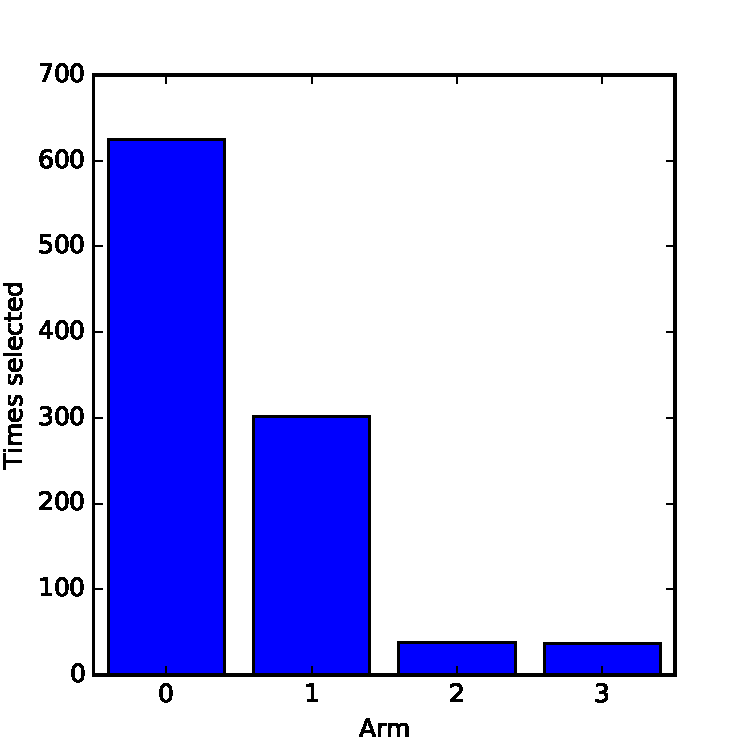
\includegraphics[width=.16\textwidth]{./fig/ex1-2-a2.pdf}}
	\subfloat[][$\epsilon$-greedy 0.2]{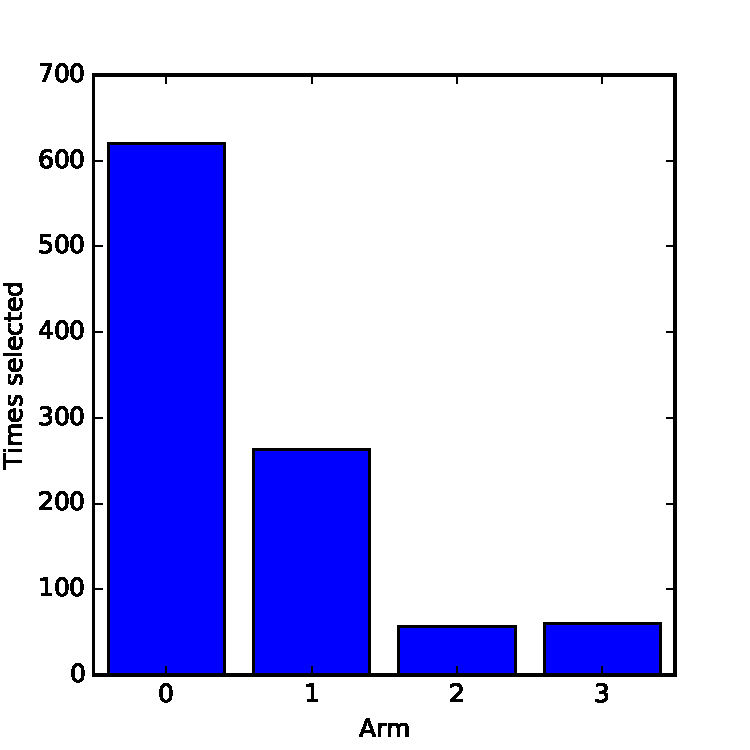
\includegraphics[width=.16\textwidth]{./fig/ex1-2-a3.pdf}}
	\subfloat[][Softmax 1]{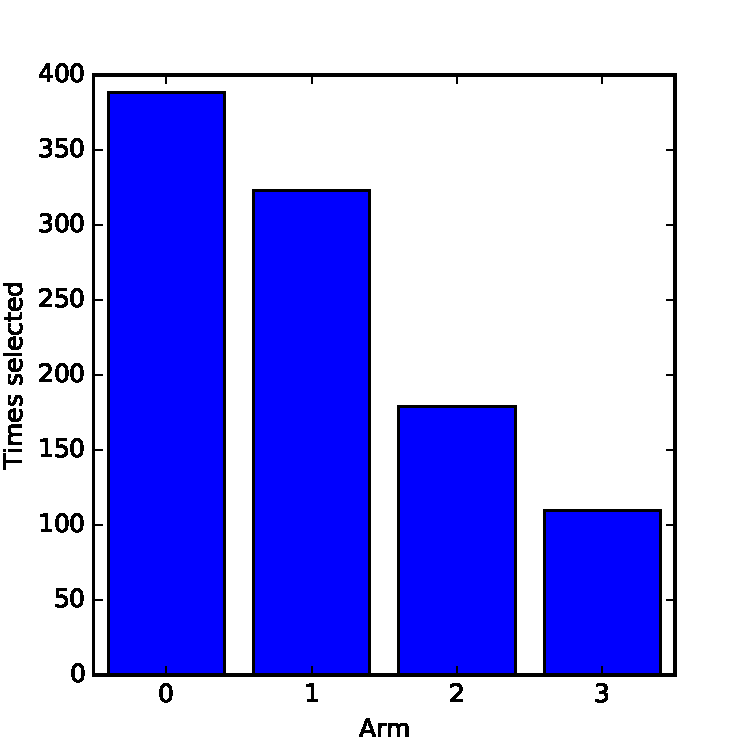
\includegraphics[width=.16\textwidth]{./fig/ex1-2-a4.pdf}}
	\subfloat[][Softmax 0.1]{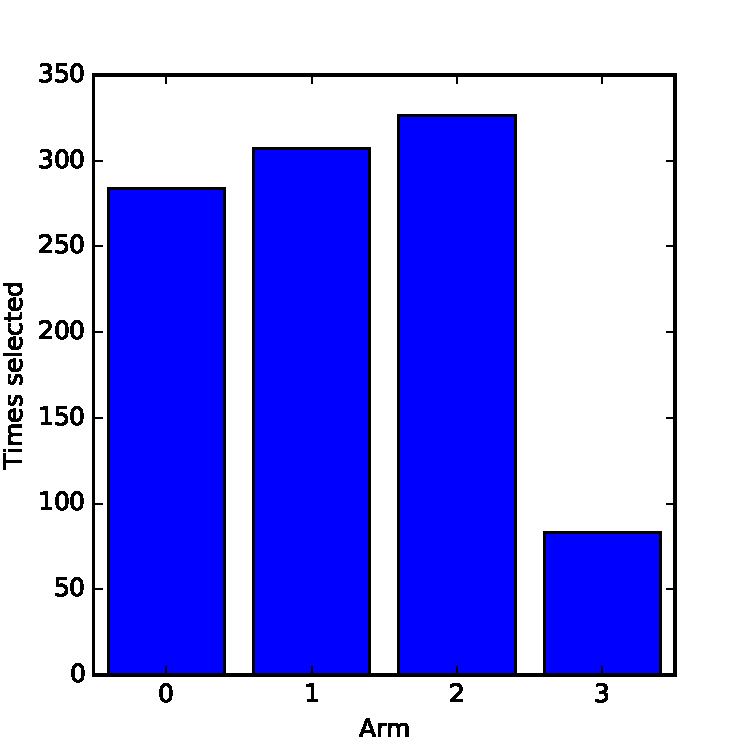
\includegraphics[width=.16\textwidth]{./fig/ex1-2-a5.pdf}}
	\caption{Actions taken by each algorithm}
	\label{ex12a}
\end{figure}

\begin{figure}[H]
	\centering
	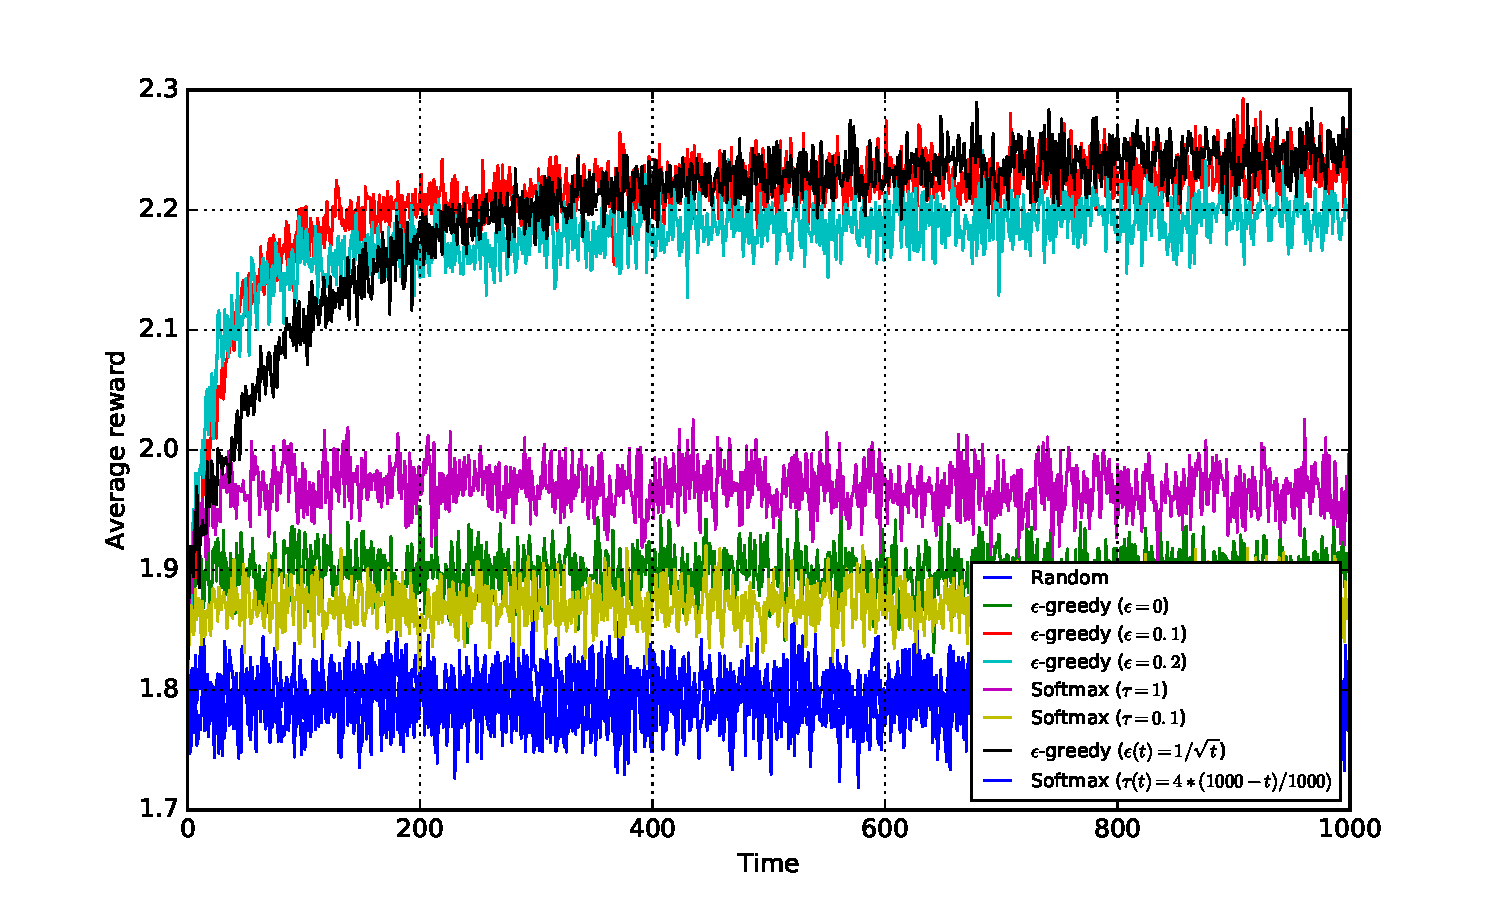
\includegraphics[width=0.7\textwidth]{./fig/ex1-3.pdf}
	\caption{Evolution of the average reward over 3000 runs during training}
	\label{ex13perf}
\end{figure}
\begin{figure}[H]
	\centering
	\subfloat[][Arm 1]{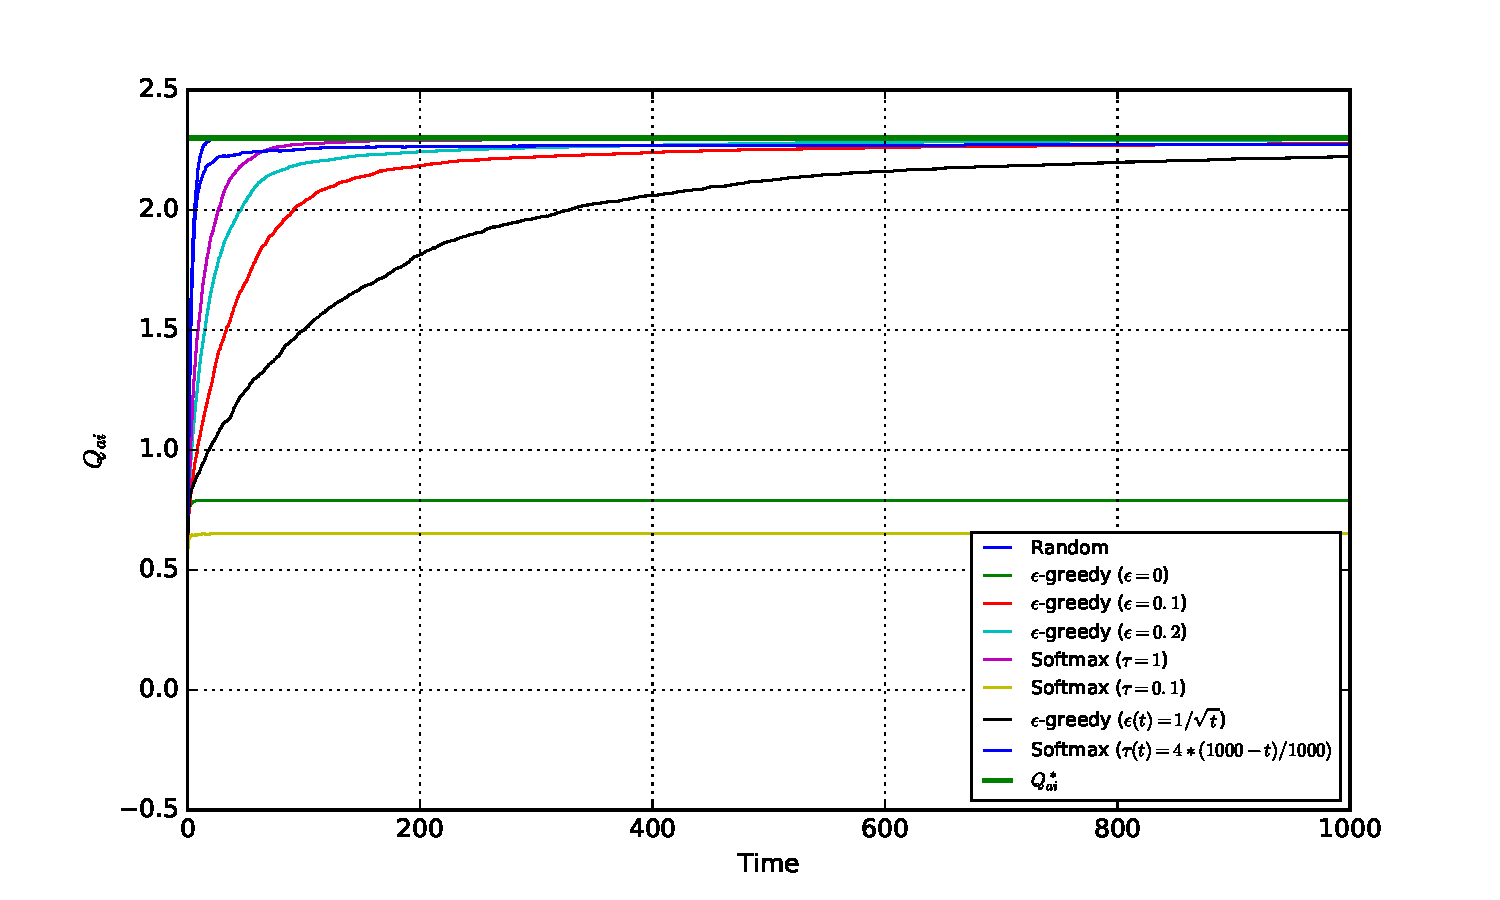
\includegraphics[width=.49\textwidth]{./fig/ex1-3-q0.pdf}}
	\subfloat[][Arm 2]{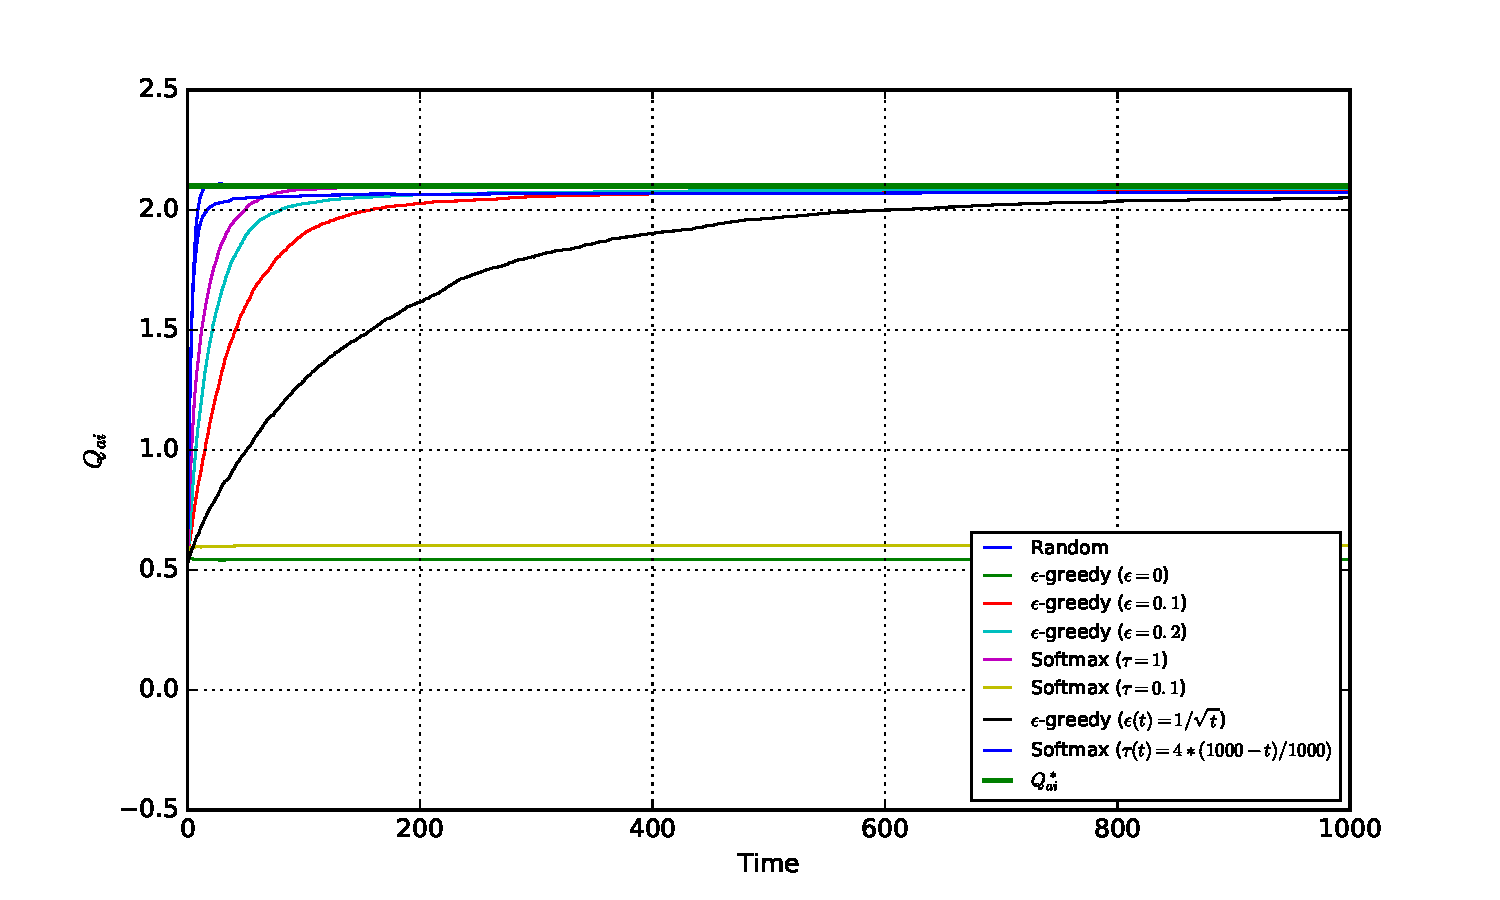
\includegraphics[width=.49\textwidth]{./fig/ex1-3-q1.pdf}}
	\\
	\subfloat[][Arm 3]{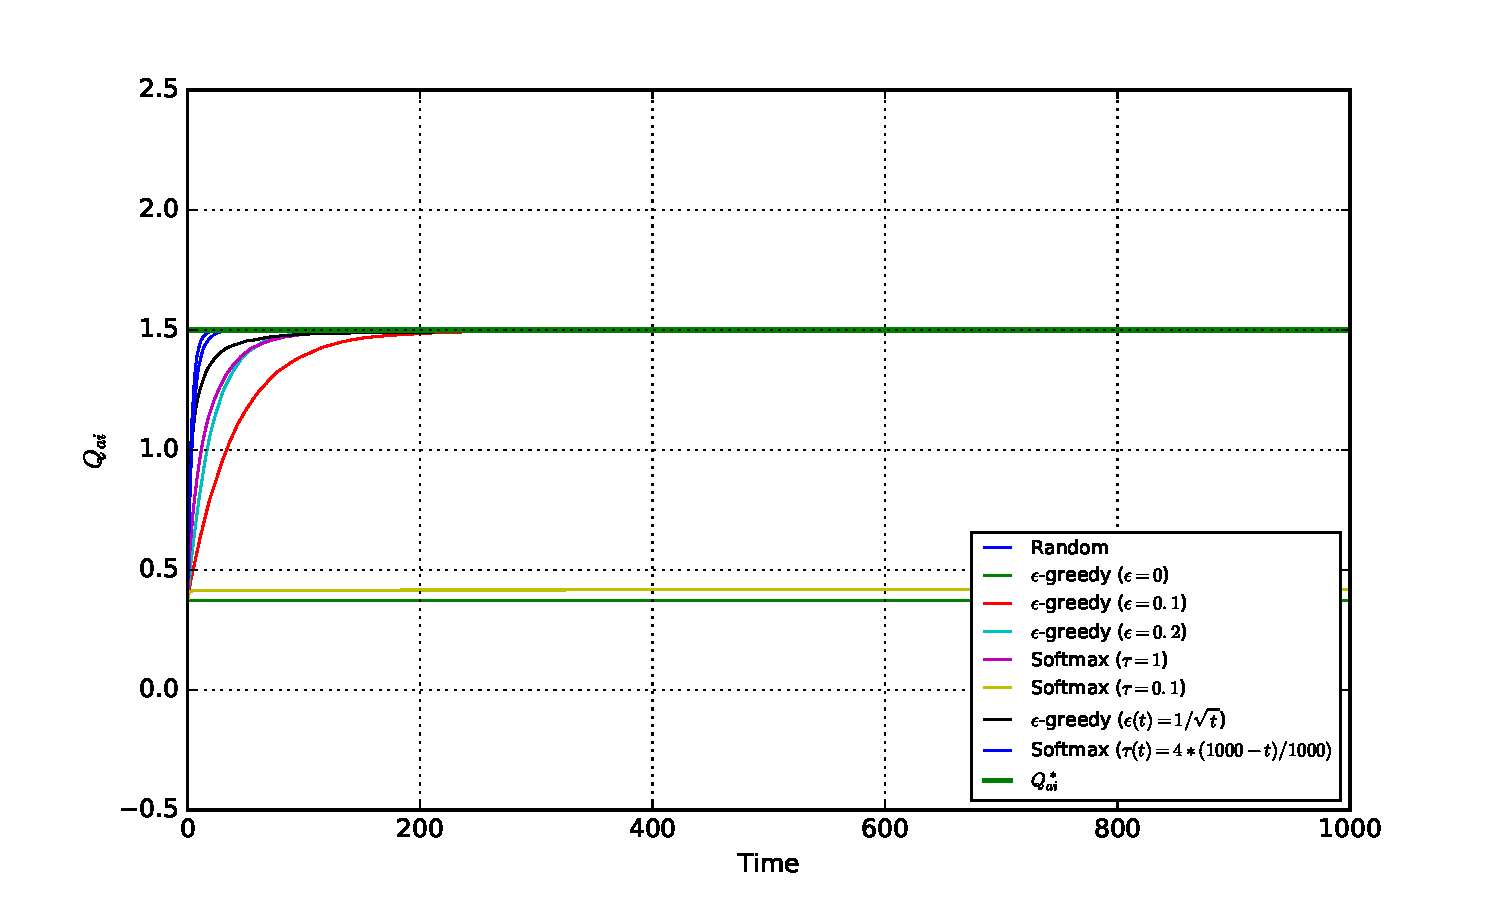
\includegraphics[width=.49\textwidth]{./fig/ex1-3-q2.pdf}}
	\subfloat[][Arm 4]{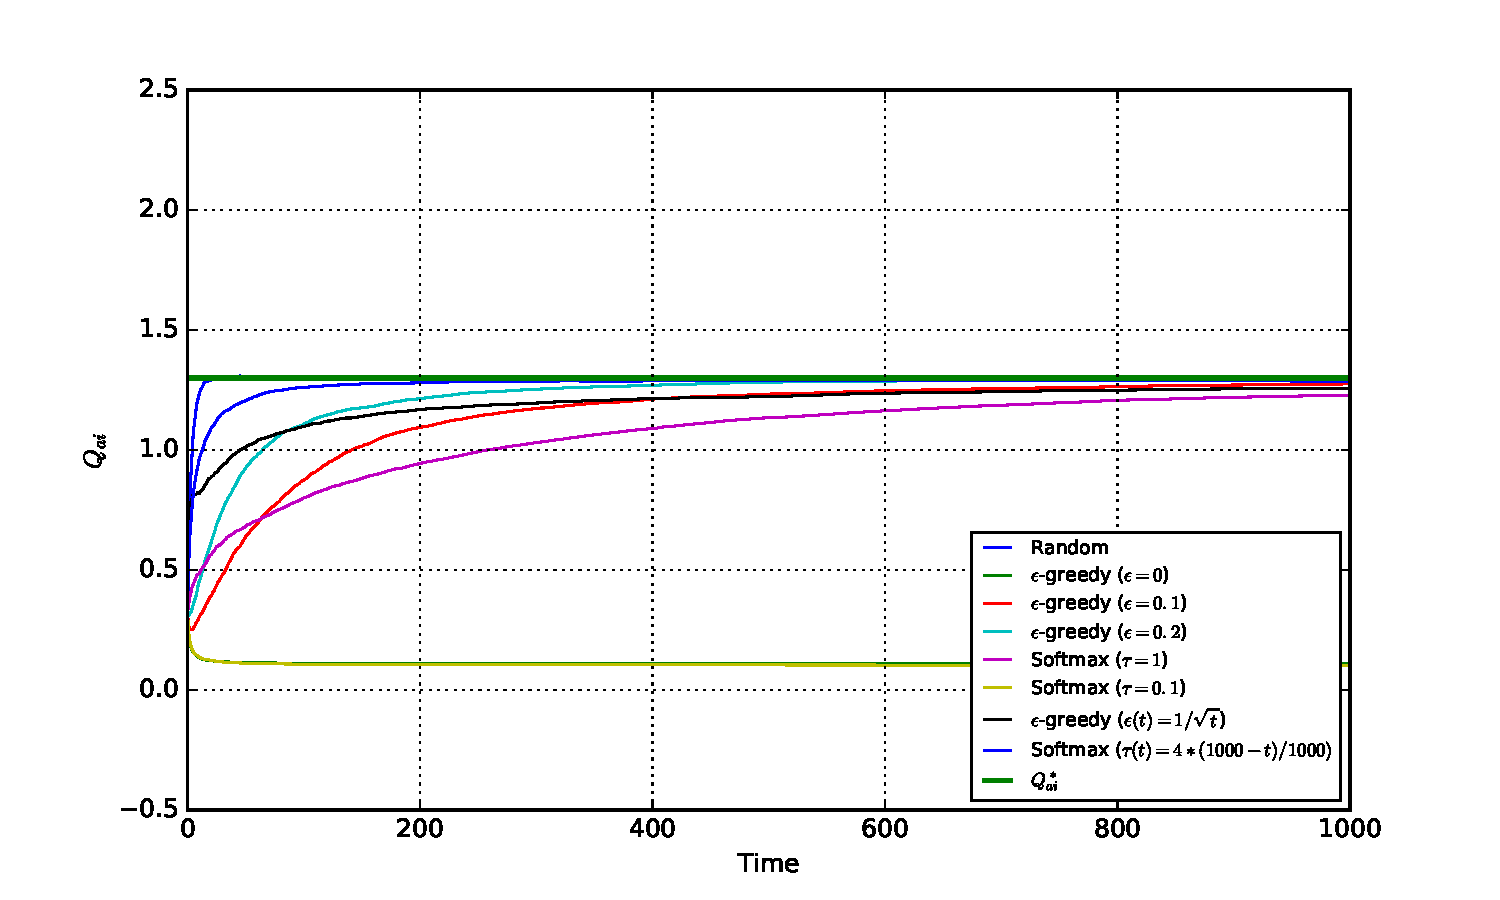
\includegraphics[width=.49\textwidth]{./fig/ex1-3-q3.pdf}}
	\caption{Evolution of $Q_{ai}$ for each arm}
	\label{ex13q}
\end{figure}
\begin{figure}[H]
	\centering
	\subfloat[][Random]{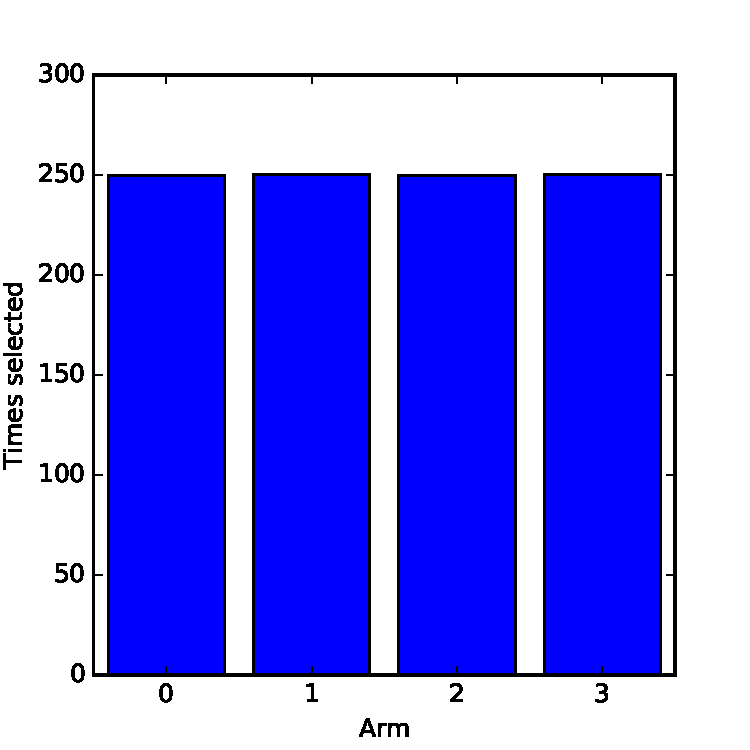
\includegraphics[width=.16\textwidth]{./fig/ex1-3-a0.pdf}}
	\subfloat[][$\epsilon$-greedy 0]{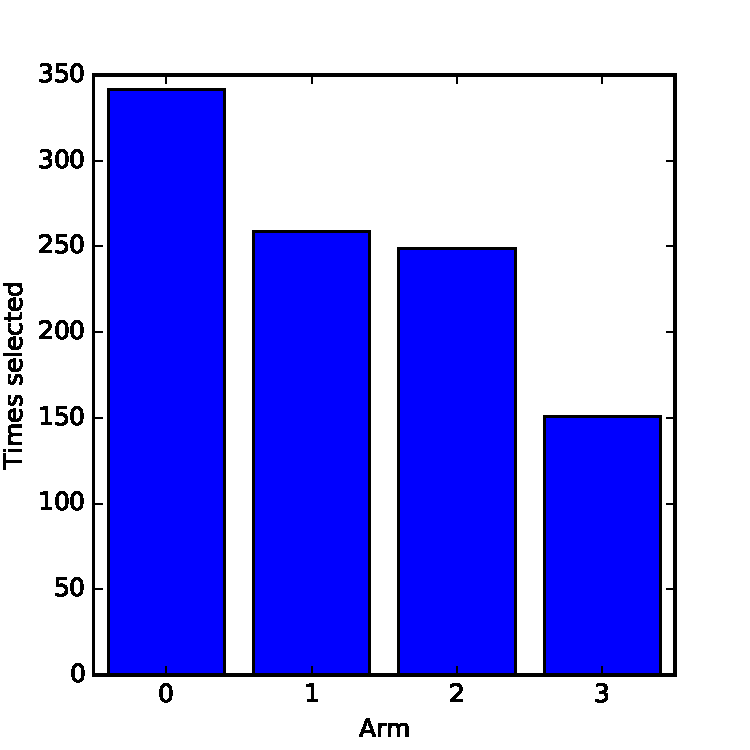
\includegraphics[width=.16\textwidth]{./fig/ex1-3-a1.pdf}}
	\subfloat[][$\epsilon$-greedy 0.1]{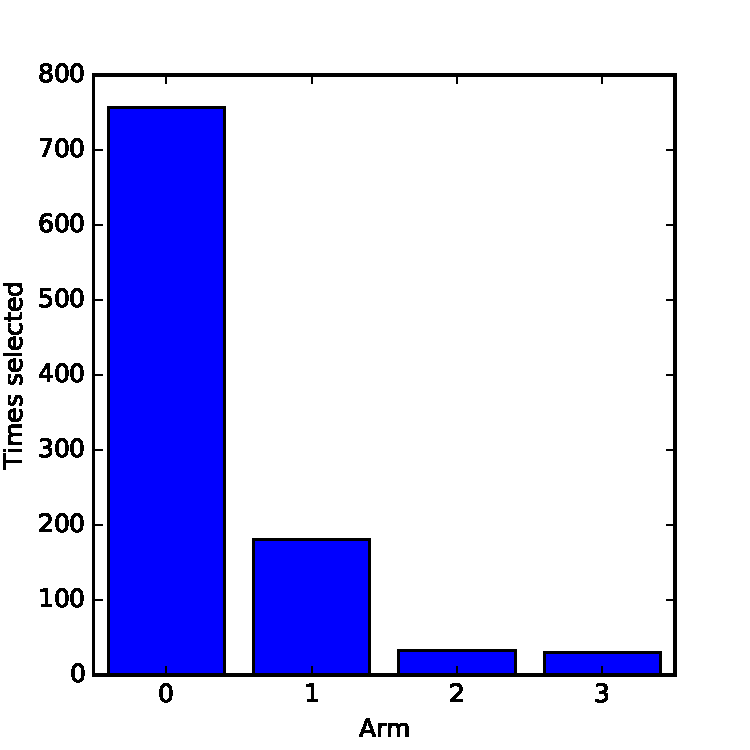
\includegraphics[width=.16\textwidth]{./fig/ex1-3-a2.pdf}}
	\subfloat[][$\epsilon$-greedy 0.2]{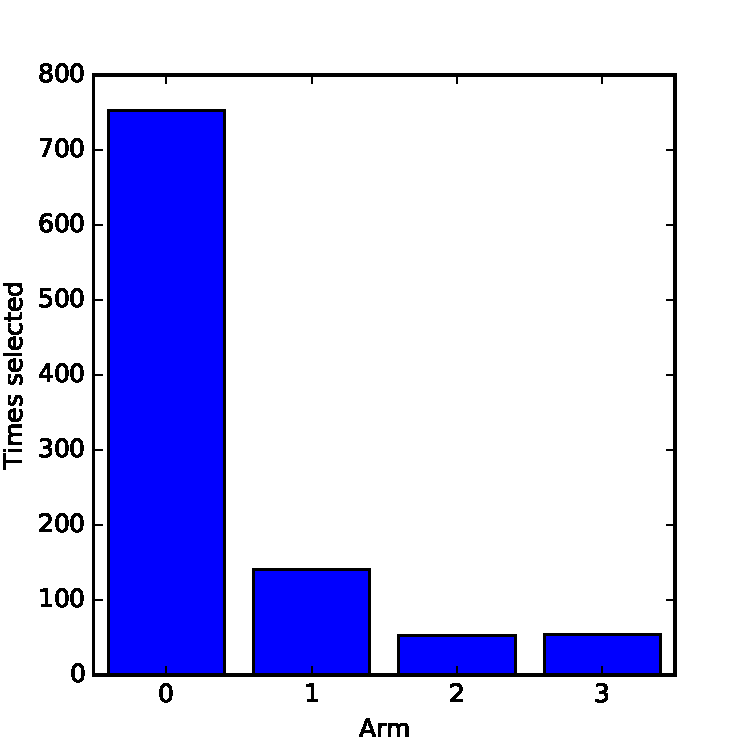
\includegraphics[width=.16\textwidth]{./fig/ex1-3-a3.pdf}}
	\\
	\subfloat[][Softmax 1]{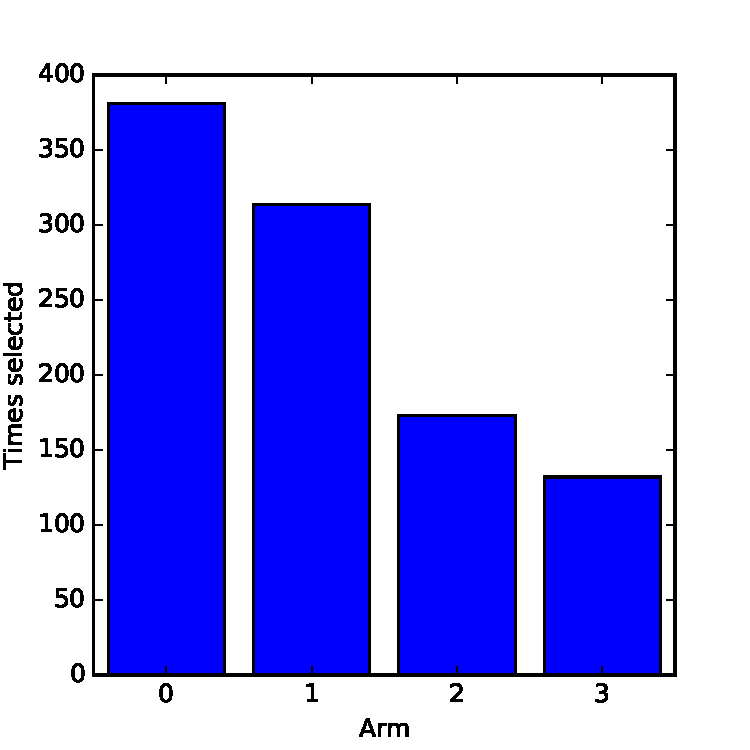
\includegraphics[width=.16\textwidth]{./fig/ex1-3-a4.pdf}}
	\subfloat[][Softmax 0.1]{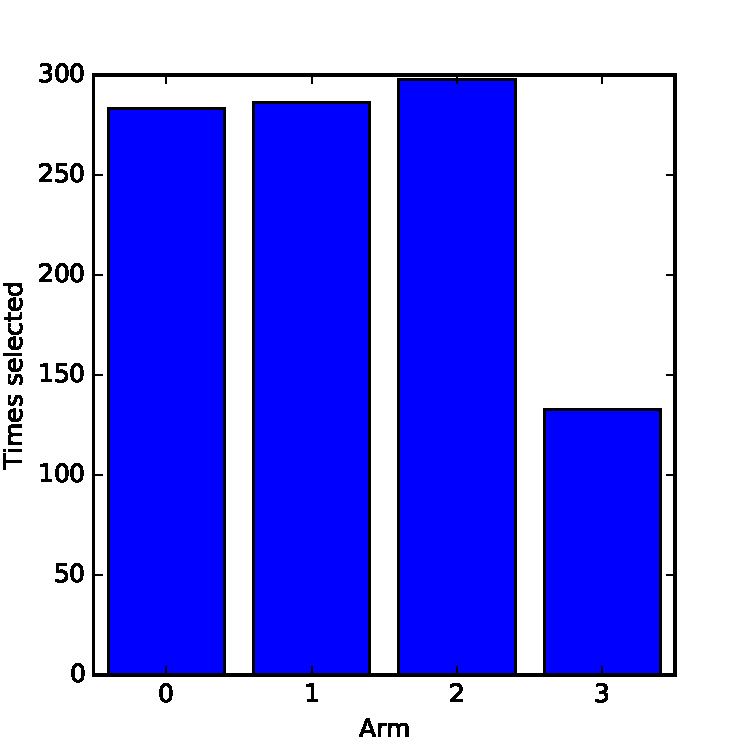
\includegraphics[width=.16\textwidth]{./fig/ex1-3-a5.pdf}}
	\subfloat[][$\epsilon(t)$]{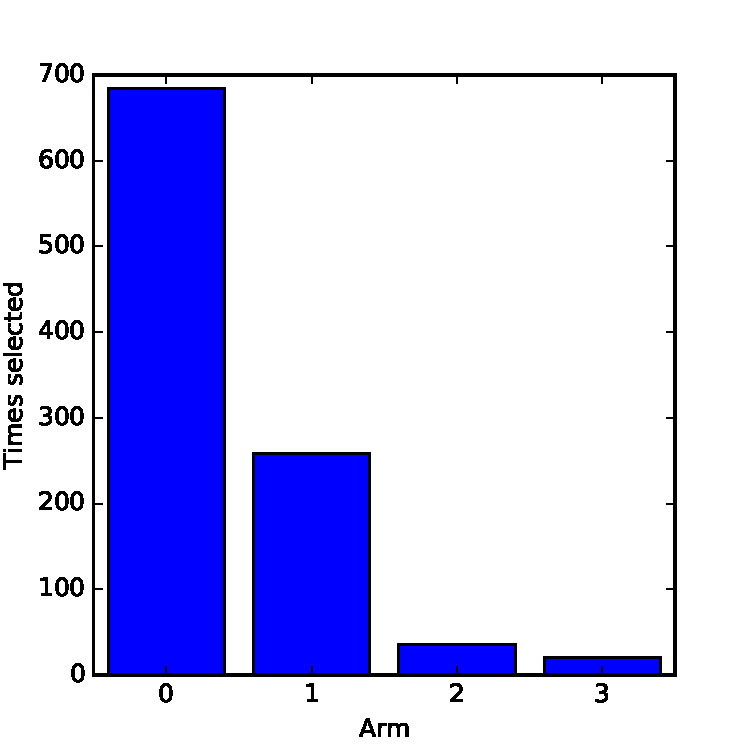
\includegraphics[width=.16\textwidth]{./fig/ex1-3-a6.pdf}}
	\subfloat[][$\tau(t)$]{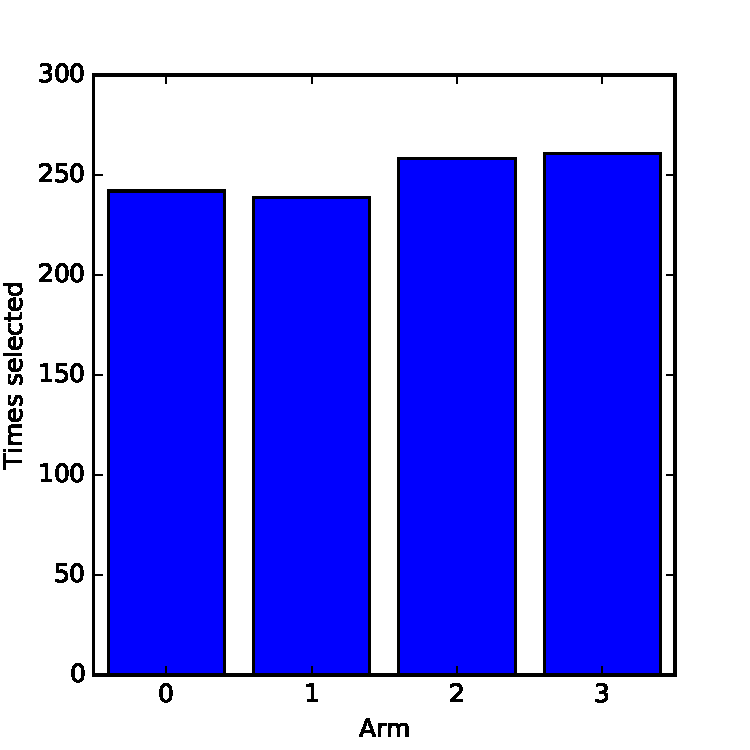
\includegraphics[width=.16\textwidth]{./fig/ex1-3-a7.pdf}}
	\caption{Actions taken by each algorithm}
	\label{ex13a}
\end{figure}
\end{document}
